\label{chp:anharmonicity}

As we have seen in the previous chapter, thermal conductivity is an anharmonic effect -- in a purely harmonic system, thermal conductivity is infinite. We have also discussed methods to assess thermal transport in materials, either via the Green-Kubo approach, or via perturbation theory, where the potential energy is expanded to third or fourth order, and these terms are used to compute the change of phonon properties, in particular, their lifetimes.\CITE{see paper}
From a computer simulation perspective, the two approaches have different strengths: Perturbative techniques are ideally suited, as the name suggest, when the anharmonicity is weak,~i.\,e.,~the harmonic terms in the potential dominate the dynamical evolution of the system. The Green-Kubo technique on the other hand does not need approximations to the potential energy surface, and therefore naturally includes all orders of anharmonicity. It is ideally suited in situations where the anharmonicity is strong,~i.\,e.,~when the basic assumption of perturbation theory is not satisfied. It is therefore desirable to \emph{measure} the ``degree of anharmonicity'' to enable a discussion of anharmonicity on a quantitative basis.

\REM{few words about grueneisen?}

\newthought{The chapter is based on work performed by the author}, as published in Ref.\,\cite{Knoop2020}. We therefore only summarize the key ideas adopted in this thesis.\REM{say sth. else?}

\section{Definition of Anharmonicity}

In accordance with the previous chapters, the classical nuclear dynamics within Born-Oppenheimer approximation are governed by the Hamiltonian
\begin{align}
	\mathcal H ( {\bf P}, {\bf R}) 
		= \sum_I \frac{\b P_I^2}{2 M_I} + \mathcal V (\b R)~,
	\label{eq:anh.H}
\end{align}
where $\bf P$ and $\bf R$ denote the atomic momenta and coordinates, as usual. Using an expansion of the the full potential $\mathcal V ({\bf R})$ in the displacements $\bf U$ around a reference configuration ${\bf R}^0$ as discussed in Chp.\,\ref{chp:dynamics}, the potential can be split into a harmonic contribution, $\mathcal V^{(2)}$, and a second term capturing all anharmonic effects, therefore termed $\mathcal V^{\rm A}$,
\begin{align}
	\mathcal V ({\bf R})
		= \mathcal V^{(2)} ({\bf R}) + \mathcal V^{\rm A} ({\bf R})~.
	\label{eq:anh.V}
\end{align}
In the classical limit, the dynamical evolution of the nuclei is determined by the potential through the atomic forces as defined Eq.\,\eqref{eq:dyn.eom.classical},
\begin{align}
	M_I \ddot{\bf R}_I
		= -\frac{\partial \mathcal V}{\partial {\bf R}_I}
		\equiv {\bf F}_I~,
\end{align}
~i.\,e.,~Newton's equations of motion. By linearity of the differential, the forces can therefore be split into harmonic and anharmonic contributions as well,
\begin{align}
	{\bf F}_I
		= {\bf F}_I^{(2)} + {\bf F}_I^{\rm A}~.
	\label{eq:anh.F}
\end{align}
The division of potential and forces into harmonic and anharmonic contributions is depicted for a one-dimensional potential in Fig.\,\ref{fig:pes_sketch_vertical}.
\begin{marginfigure}
	\centering
	% 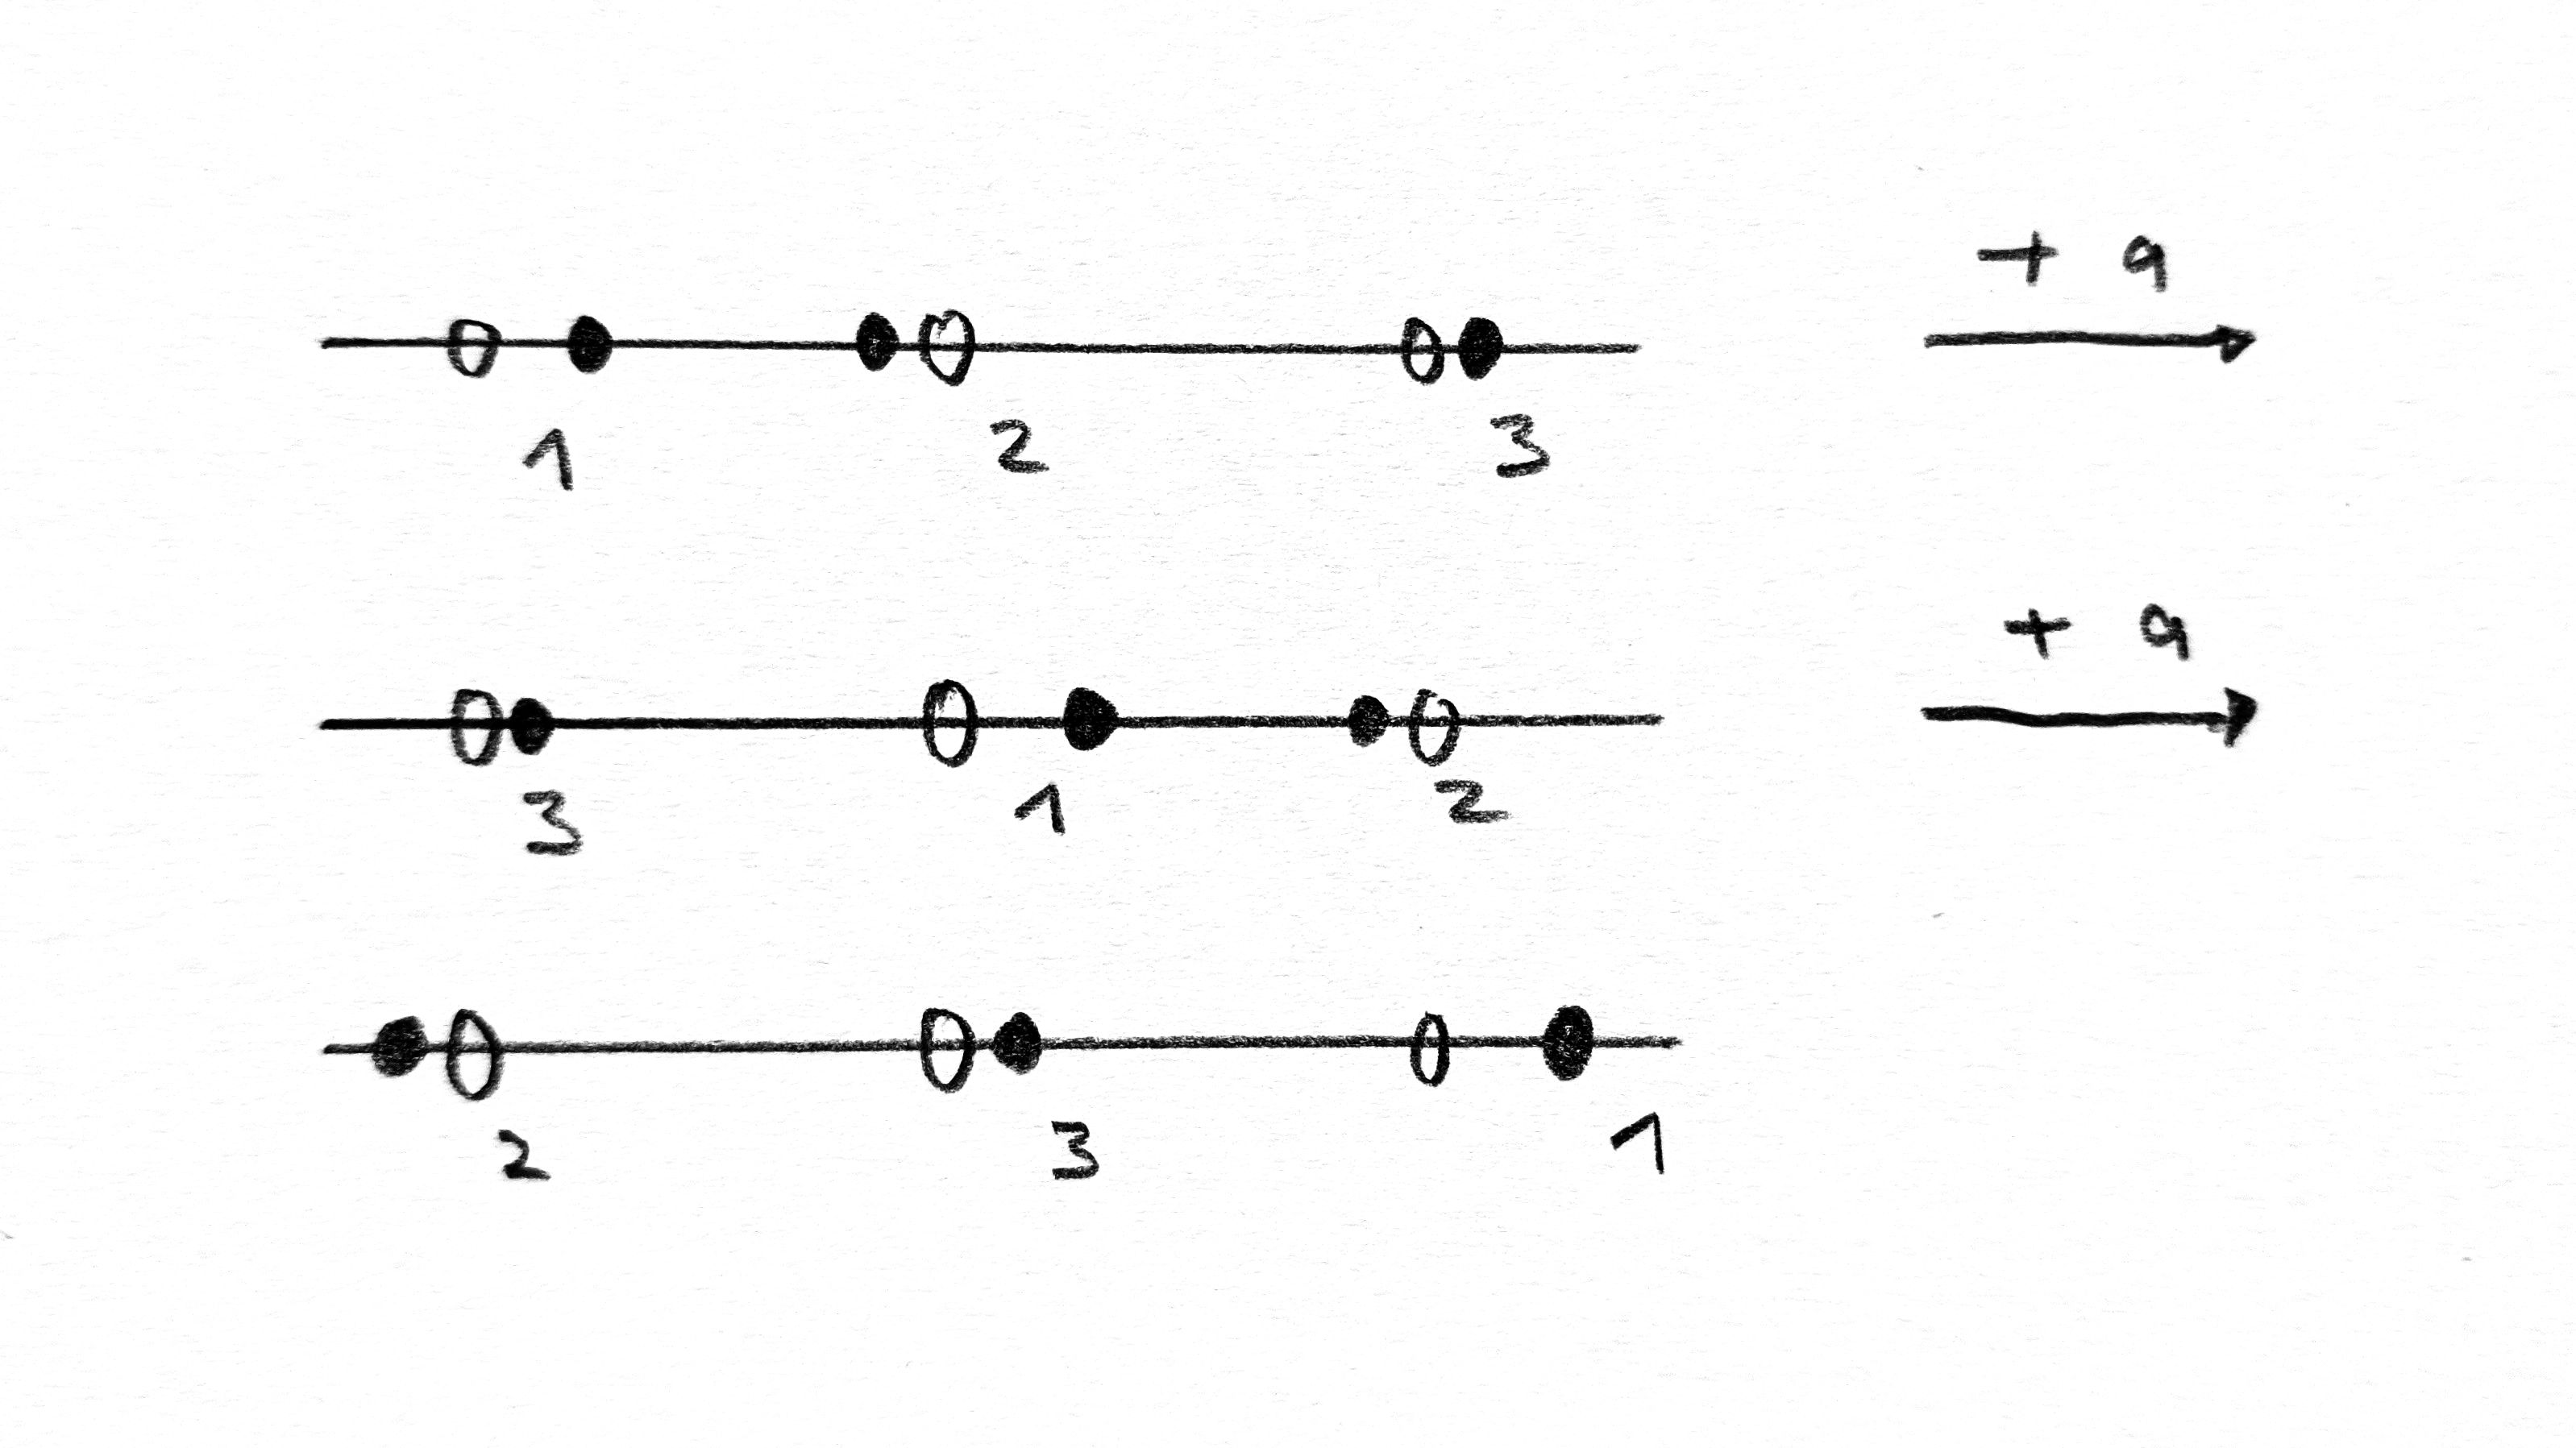
\includegraphics[width=.68\textwidth]{./sketches/permutation1.jpg}
	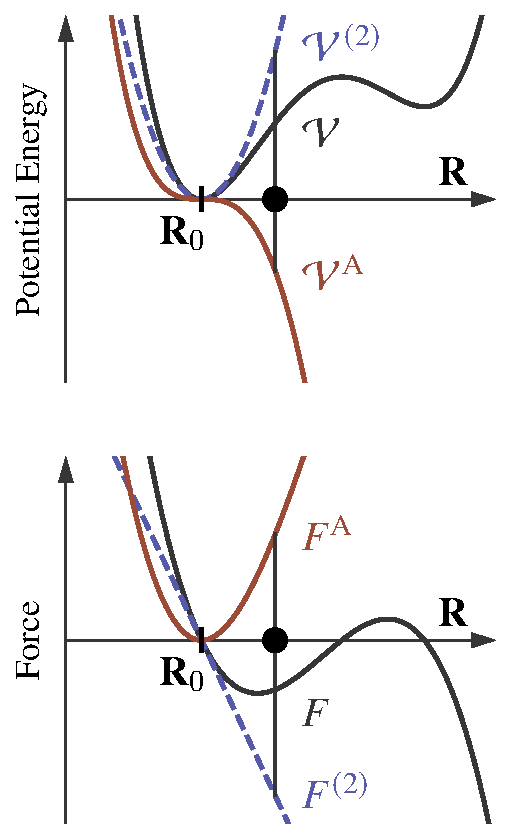
\includegraphics[width=\textwidth]{./data/plots/anharmonicity/1_pes_sketch/sketch_vertical.pdf}
	\caption{Upper: Sketch of a one-dimensional potential-energy surface $\mathcal V$ (solid black), its harmonic approximation $\mathcal{V}^{(2)} (\b R)$ (dashed blue), and the anharmonic contribution $\mathcal{V}^{\rm A} (\b R)$ (solid red). Right: The force ${F} ({\bf R})$ given by the derivative of the potential energy $\mathcal V$ (black), the force $F^{(2)}$ stemming from the harmonic potential $\mathcal{V}^{(2)} (\b R)$ (blue), and the anharmonic contribution $F^\mathrm{A} = F - F^{(2)}$ (red), cf.~Eq.\,\eqref{eq:anh.F}.}
	\label{fig:pes_sketch_vertical}
\end{marginfigure}


\section{Anharmonicity measure}

We base the definition of a measure for anharmonicity on the forces, for three reasons: First, because we have just seen that the dynamical evolution of the system is determined by the potential through the equations of motion, and therefore by the forces. Second, because the forces give more microscopic insight, as they can be resolved per atom. Third, the forces are   statistically easier to describe, since per configuration $\bf R$, there are $3N$ force components ${\bf F} = ({\bf F}_1, \ldots, {\bf F}_N)$.

In terms of the force contributions defined in Eq.\,\eqref{eq:anh.F}, we define a \emph{measure of anharmonicity} in the following way:
\begin{align}
	\sigmaA (T)
		% = \frac{\sigma [F^{\rm A}]_T}{\sigma [F]_T}
		= \sqrt{\frac{\sum_{I, \alpha} \braket{(F^{\rm A}_{I, \alpha})^2}_T}{\sum_{I, \alpha} \braket{(F_{I, \alpha})^2}_T}}~,
	\label{eq:sigmaA}
\end{align}
where $F_{I, \alpha}^{(A)}$ is the $\alpha$ component of the (anharmonic) force on atom $I$, and $\braket{\cdot}_T$ denotes a thermodynamic average at temperature $T$. The interpretation of the measure $\sigmaA$ is that it quantifies the anharmonic strength in terms of the standard deviation of the distribution of anharmonic force components at a given temperature, $\sigma [F^{\rm A}]_T$, normalized by the standard deviation of the actual force distribution, $\sigma [F]_T$, where the standard deviation of force distribution is defined as
\begin{align}
	\sigma [F]_T 
		= \sqrt{\frac{1}{3N} \sum_{I, \alpha} \braket{F_{I, \alpha}^2}_T}~.
\end{align}
The effect of normalizing the distribution of forces is shown in Fig.\,\ref{fig:anh.normalization} for the two exemplary materials already discussed in the context of phonon dispersions in Sec.\,\ref{sec:ha.dispersions}, fcc-silicon, and the orthorombic perovskite KCaF$_3$. Only after normalizing the forces, a meaningful comparison between materials or across temperatures can be achieved.
\begin{marginfigure}
	\centering
	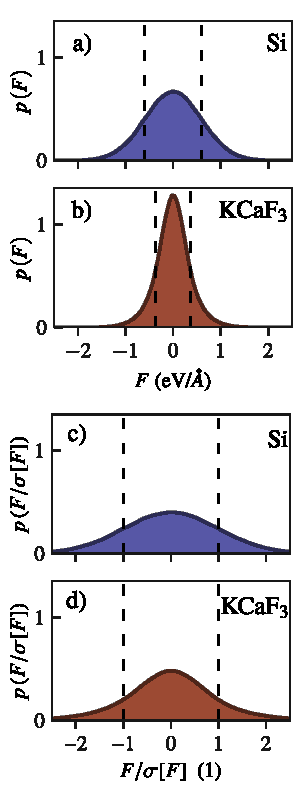
\includegraphics[width=0.8\textwidth]{./data/plots/anharmonicity/4_force_distribution/histogram_forces_vertical.pdf}
	\caption{
		Force component distribution before and after normalization with the width of the distribution $\sigma [F]$. $p(F)$ denotes the probability to find a force component $F_{I, \alpha}$ of strength $F$ in the material. Panel a) and b) show the distribution before normalization, c) and d) after normalization. Dashed vertical lines denotes the standard deviation of the displayed distribution.
	}
	\label{fig:anh.normalization}
\end{marginfigure}


\newthought{For the two exemplary materials, we show the joint normalized distributions of force and anharmonic force contributions} in Fig.\,\ref{fig:anh.sigmaA}.
\begin{figure}
	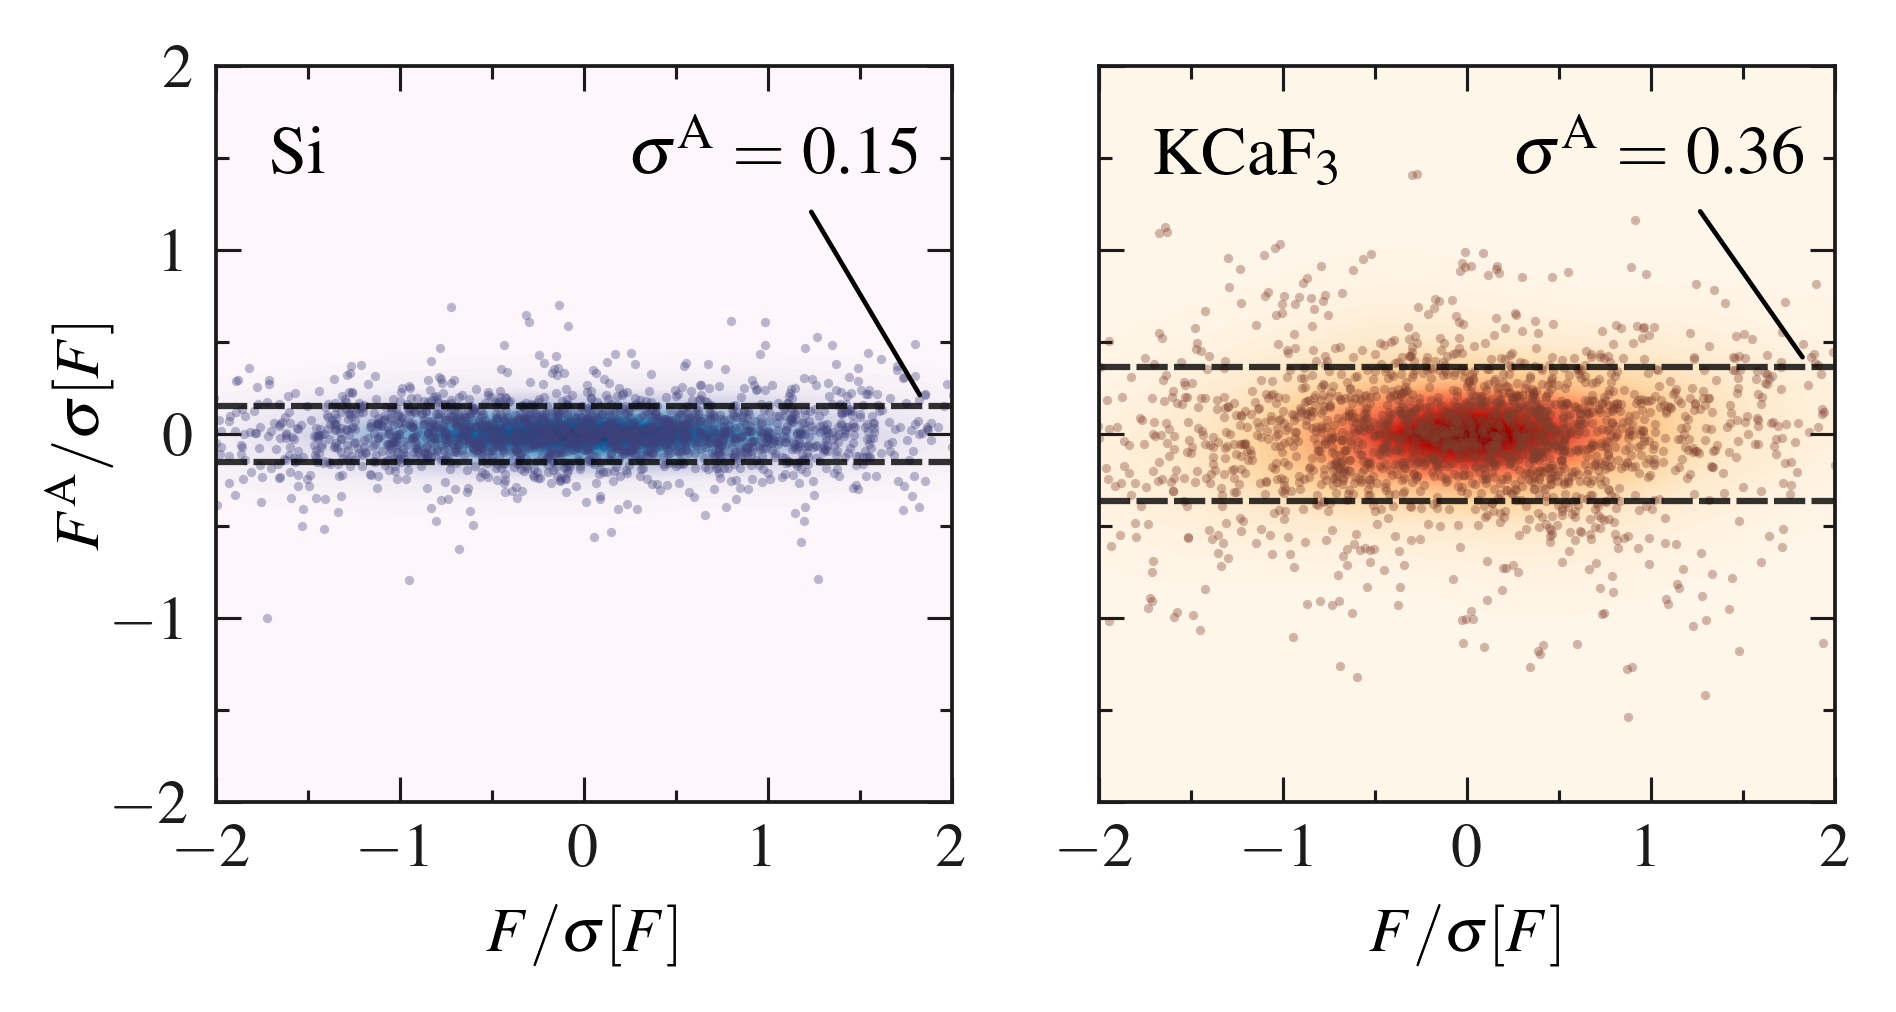
\includegraphics[width=\textwidth]{./data/plots/anharmonicity/5_density_plots/histogram_annotated.png}
	\caption{
		Normalized anharmonic force components versus normalized force components. Dashed horizontal lines: Width of the distribution estimated from standard deviation. Individual dots are force components sampled during an \emph{ab initio} MD simulations.
	}
	\label{fig:anh.sigmaA}
\end{figure}
In this representation, the measure of anharmonicity $\sigmaA$ is given by the standard deviation of the distribution in y-direction, as indicated by the dashed horizontal lines in the plot. The distribution of anharmonic force components is more than twice as broad for the perovskite KCaF$_3$ compared to silicon, with a $\sigmaA$ of 0.36 compared to 0.15, respectively. This can be interpreted in the sense that 36\,\% of the forces stem from anharmonic contributions in KCaF$_3$, and 15\,\% in silicon. Furthermore, strongly anharmonic force contributions with a strength of $0.5\,\sigma [F]$ or more are nearly absent in silicon with a probability of $<0.01\,\%$, whereas anharmonic forces of this strength in KCaF$_3$ occur with a much higher probability of $\sim 16.5\,\%$.


\newthought{The anharmonicity measure defined in Eq.\,\eqref{eq:sigmaA}} can also be evaluated for subsets of the dynamical degrees of freedom,~e.\,g.,~per chemical species, as shown in Fig.\,\ref{fig.anh.sigmaA.atoms}.
\begin{figure}
	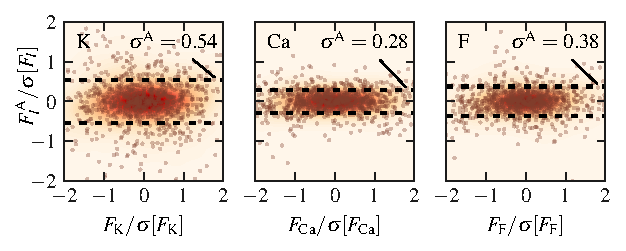
\includegraphics[width=\textwidth]{./data/plots/anharmonicity/5_density_plots/histogram_atoms.pdf}
	\caption{
		Normalized anharmonic force components versus normalized force components. Dashed horizontal lines: Width of the distribution estimated from standard deviation.
	}
	\label{fig.anh.sigmaA.atoms}
\end{figure}
In the example of KCaF$_3$, this analysis shows that the calcium (Ca) atoms occupying the vertices of the unit cell are comparatively well described by the harmonic model, whereas the description of potassium (K) is particularly bad. This can be explained by the phase-transition mechanism observed in KCaF$_3$: Above 560\,K, the material becomes cubic, and the octahedral displacement of fluorine~(F) is removed, as shown in Fig.\,\ref{fig:anh.KCaF3}. This tilt also affects the potassium atoms, which are displaced from their high-temperature reference position in the orthorombic phase, and are therefore located in a shallow potential~\cite{Bulou1980,Hidaka1984}.
\begin{marginfigure}
	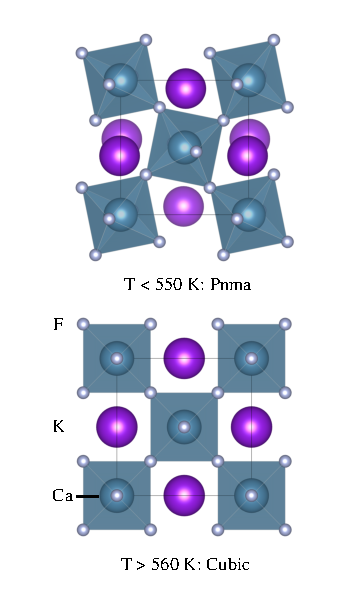
\includegraphics[width=\textwidth]{./data/plots/anharmonicity/2_materials/both.pdf}
	\caption{
		\label{fig:KCaF3}
		KCaF$_3$ in the low-temperature Pnma~(top) and high-temperature cubic phase~(bottom). Both structures are viewed along the long $b$-axis.
	}
	\label{fig:anh.KCaF3}
\end{marginfigure}

\newthought{Furthermore, it is instructive to evalute the anharmonicity for single configurations}, be it snapshots in time during molecular dynamics simulations, or when using other sampling approaches,~e.\,g,~harmonic Monte Carlo samples as defined in Eq.\,\eqref{eq:ha.samples}. While we will discuss ``time-resolved anharmonicity'' in detail at a later point, we show the evaluation of $\sigmaA$ for samples generated by Eq.\,\eqref{eq:ha.samples} in Fig.\,\ref{fig:anh.sampling}.
\begin{figure}
	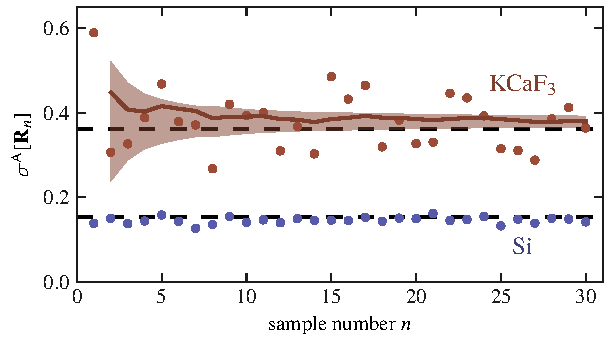
\includegraphics[width=4.1in]{./data/plots/anharmonicity/7_sampling/convergence_sigma_MC.pdf}
	\caption{
			Anharmonicity measure $\sigmaA$ evaluated for individual atomic configurations obtained from Eq.\,\eqref{eq:ha.samples}. Dots: $\sigmaA [{\bf R}_n]$ for individual samples; Red line: Cumulative average.	Black dashed line: $\sigmaA$ from \emph{ai}MD.	Shadowed region: Convergence estimated by standard error.
	}
	\label{fig:anh.sampling}
\end{figure}
The analysis shows that a decent estimate of the anharmonicity measure $\sigmaA$ can be obtained from the harmonic sampling analysis with few samples. Especially in silicon, each individual harmonic sample yields a $\sigmaA$ within 99\,\% of the reference value obtained by MD simulations for several hundred simulation time steps, which is indicated by the dashed vertical line. For the more anharmonic KCaF$_3$, the harmonic sampling with 30~samples yields an estimated value of $\sigmaA_{\rm est.} = 0.38$, which differs from the MD value ($\sigmaA = 0.36$) by about 5\,\%. A distinction between largely harmonic materials like silicon, and anharmonic materials like KCaF$_3$, is therefore possible with very few samples.

\newthought{Motivated by this fact, we investigated the possiblity to estimate $\sigmaA$ based on a single sample}, as suggested by Zacharias and coworkers in Ref.\,\cite{Zacharias2016}, where a single, deterministic sample probing the most probable part of the harmonic distribution is used by choosing $\zeta_s = (-1)^s$ instead of a random distribution in Eq.\,\eqref{eq:ha.samples}. We denote anharmonicity measures obtained by such a ``one-shot'' approach by $\sigmaAOS$ in the following. As shown in Fig.\,\ref{fig:anh.one-shot}, the one-shot samples provide very good estimates for silicon in the the entire temperature range from 200\,K to 800\,K, which can be expected due to the largely harmonic nature of silicon.
\begin{figure}
	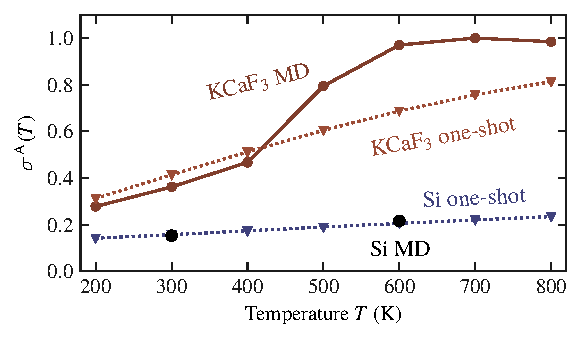
\includegraphics[width=4.1in]{./data/plots/anharmonicity/7_sampling/sigma_temp_one_shot.pdf}
	\caption{
		$\sigmaA$ as a function of temperature obtained from MD~simulations (black circles) and one-shot sampling (triangles connected by dashed curves)
	}
	\label{fig:anh.one-shot}
\end{figure}
For KCaF$_3$, the agreement is good in the temperature range from 200\, to 400\,K, at least within the limits of the harmonic sampling approach as discussed in the previous paragraph, taking into account that only a single sample was used. Above 500\,K, however, the difference to the reference value from MD simulations increases, which is due to the phase transition mechanism in KCaF$_3$ discussed earlier: This phase transition also occurs in the simulation cell. A prediction of anharmonicity across phase transitions therefore cannot be expected from simple harmonic sampling approaches, because the entire reference frame for the harmonic model changes when a phase transition occurs. The phase transition mechanism of KCaF$_3$ and implications for the anharmonicity measure are further discussed in Ref.\,\cite{Knoop2020}.

\newthought{Ultimately, the applicability of the one-shot sampling approach} needs to be assessed for a diverse set of materials, especially if one aims to use this scheme to screen for anharmonicity in material space. As shown in Fig.\,\ref{fig:anh.screening} for a set of 63~materials, the one-shot sampling is reliable within $\pm 10\,\%$ for all materials in the set, up to a value of about $\sigmaA \simeq 0.3$.
\begin{figure}
	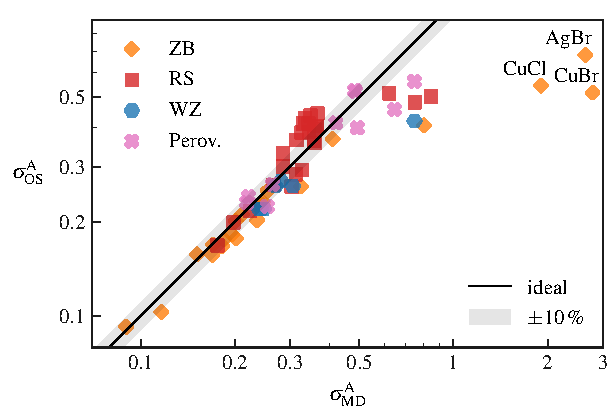
\includegraphics[width=4.1in]{./data/plots/anharmonicity/8_screening/sigma_os_md.pdf}
	\caption{
		Comparison of the anharmonicity measure obtained from MD simulations and one-shot sampling (OS) for 63 materials at 300\,K. The set comprises 25 rock salt (RS), 21 zincblende (ZS), 7 wurtzite (WZ), and 10 orthorombic perovskite (Perov.) materials. The diagonal line denotes perfect agreement between MD and OS, and the green area denotes a 10\,\%~error margin to guide the eye.
		Data was taken from Ref.\,\cite{Knoop2020}.
	}
	\label{fig:anh.screening}
\end{figure}
For larger values of $\sigmaA$, the deviation can become larger, especially for the rock salt materials with $\sigmaA \simeq 0.35$ where the one-shot sampling overestimates $\sigmaA$ by about 20\,\%. Nevertheless, the agreement is qualitatively correct up to values of about $\sigmaA \simeq 0.5$, after which materials begin to show effects not captured by the harmonic sampling,~e.\,g.,~phase transitions as discussed earlier for KCaF$_3$. In particular, the three highlighted noble metal halides AgBr, CuCl, and CuBr deviate strongly. These materials tend towards non-perturbative effects during the MD simulation such as spontaneous defect formation~\cite{Knoop2020}, which is a dynamical effect impossible to be described by any reference harmonic model. We will discuss the nature of these effects in more detail later. To conclude, we point out that also in the case of non-trivial dynamical effects such as defect formation, the estimated anharmonicity scores $\sigmaAOS$ are larger than $\gtrapprox 0.5$, and therefore indicate strong anharmonicity. A qualitative classification of strong anharmonicity in terms of one-shot sampling is therefore possible for all materials in the set, while quantitative agreement is only achieved for harmonic materials with $\sigmaA \lesssim 0.2$.


\section{Anharmonicity and thermal conductivity}

Based on the qualitative discussion of thermal transport in Sec.\,\ref{sec:hf.kappa.ha}, one can expect that stronger anharmonicity leads to shorter phonon lifetimes and therefore lower thermal conductivity. We tested this hypothesis for a list of 47 materials where experimental reference was available~\cite{Morelli2006,Chen2019}. The results are shown in Fig.\,\ref{fig:anh.kappa}.
\begin{figure}
	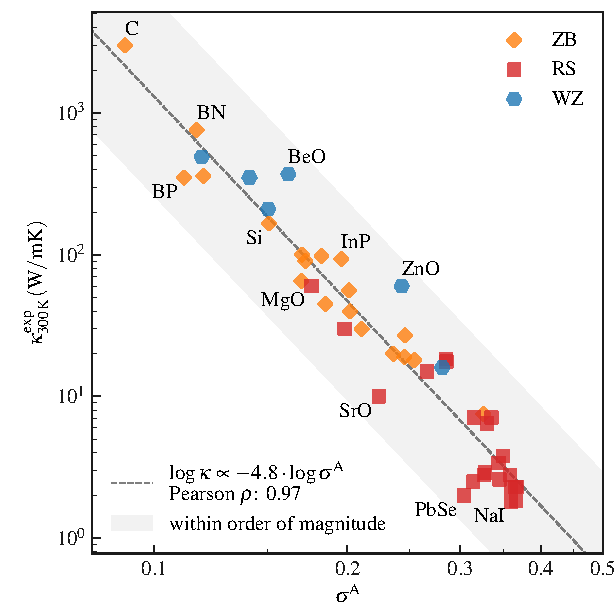
\includegraphics[width=4.1in]{./data/plots/anharmonicity/9_kappa/sigma_vs_kappa.pdf}
	\caption{
		Experimental thermal conductivity at room temperature, $\kappa^{\rm exp}_{300\,{\rm K}}$, versus one-shot measure of anharmonicity, $\sigmaAOS$. The dashed diagonal line indicates a power law fit for the data. The grey area denotes values of $\kappa$ which agree with the fit within an order of magnitude. The dataset contains 47 materials, 22 rock salt (RS), 19 zincblende (ZB), and 6 wurtzite (WZ) structures. Experimental data from Ref.~\cite{Morelli2006,Chen2019}.
	}
	\label{fig:anh.kappa}
\end{figure}
The analysis reveals an inverse power law relationship between thermal conductivity and anharmonicity for the materials in the dataset. Given that just a single descriptor was used,~i.\,e.,~the estimated anharmonicity score, and no further vibrational properties as commonly employed in semi-empirical models for thermal condcutivity\CITE{Curtarolo,Toberer,Ramprasad}, this observation is somewhat surprising. At the same time, the inverse correlation is an indication that $\sigmaA$ indeed captures some essential physics relevant to heat transport.

\newthought{The most important messages from Fig.\,\ref{fig:anh.kappa} can be summarized as follows}, adopting the definition suggested by Morelli and Slack to define ``high thermal conductivity'' as $\kappa \gtrsim 50 \, {\rm W/mK}$~\cite{Morelli2006}:
\begin{enumerate}
	\item Largely harmonic materials with $\sigmaA \simeq 0.1$, like diamond (C), boron nitride (BN), or boron phosphide (BP) can be expected to be good thermal conductors with $\kappa \gtrsim 100\,{\rm W/mK}$.
	\item Strongly anharmonic materials with $\sigmaA \gtrsim 0.3$ can be expected to be poor thermal conductors with $\kappa \lesssim 10\,{\rm W/mK}$.
	\item $\sigmaA$ has a strong correlation with thermal conductivity across the entire dataset, but nevertheless only a rough estimate can be made solely based on $\sigmaA$, especially in the middle region with $\sigmaA \simeq 0.2$. This can be seen by comparing strontium oxide (SrO) with $\kappa = 10\,{\rm W/mK}$ and $\sigmaA = 0.22$, and zinc oxide (ZnO) with $\kappa = 60\,{\rm W/mK}$ and $\sigmaA = 0.24$, or beryllium oxide (BeO) with $\kappa = 370\,{\rm W/mK}$ and $\sigmaA = 0.16$ to magnesium oxide (MgO) with $\kappa = 60\,{\rm W/mK}$ and $\sigmaA = 0.18$. These pairs of materials differ only slightly in their estimated anharmonicity, but still quite strongly in the thermal conductivity. 
\end{enumerate}

\newthought{These findings suggest the following approach} towards screening material space in search for thermal insulators: Estimate the anharmonicity for materials of interest and discard the largely harmonic ones, as they will be good thermal conductors most of the time. Of course, the reverse approach can be pursued when searching for materials with potentially high thermal conductivity.

\section{Candidate Materials}
\begin{marginfigure}
	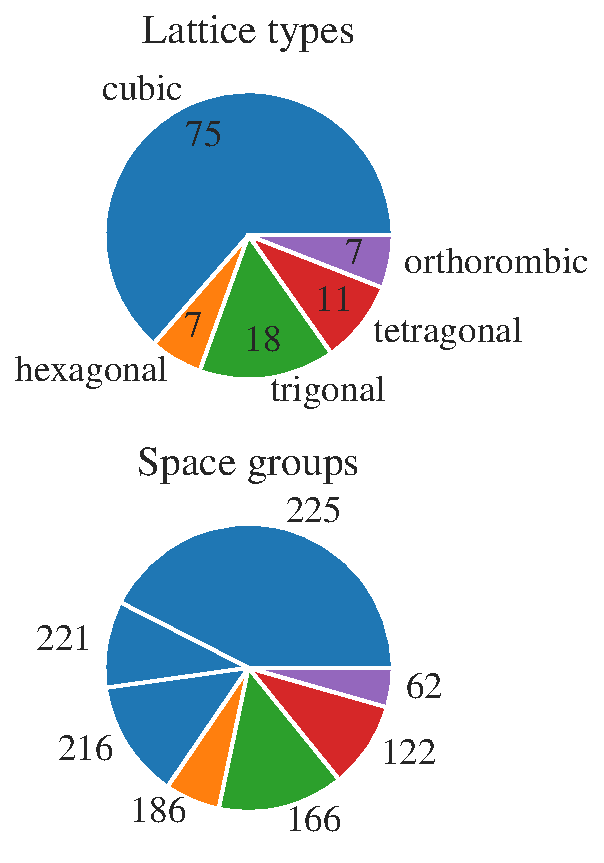
\includegraphics[width=\textwidth]{./data/plots/dataset/pies.pdf}
	\caption{
		Lattice types and space groups represented in the dataset. Space groups not shown in the pie chart: 56, 61, 160, 164, 206, with one representative each.
	}
	\label{fig:anh.pie}
\end{marginfigure}
In the context of the work published in Ref.\,\cite{Knoop2020}, we have identified a set of 118 binary and ternary materials for further investigation with the \emph{ab intio} Green Kubo (aiGK) approach. The materials comprise five lattice types and 12 space groups as summarized in Fig.\,\ref{fig:anh.pie}.  Since we are mainly interested in thermal insulators as candidate thermoelectric and thermal barrier coating materials, we have discarded largely harmonic materials with $\sigmaA < 0.17$ from the set, and focus on anharmonic strengths $\sigmaA > 0.2$ with a mean of $\sigmaA=0.31$ and a median of $\sigmaA = 0.29$. A histogram displaying the distribution of $\sigmaA$ values is shown in Fig.\,\ref{fig:anh.histogram}.
\begin{figure}
	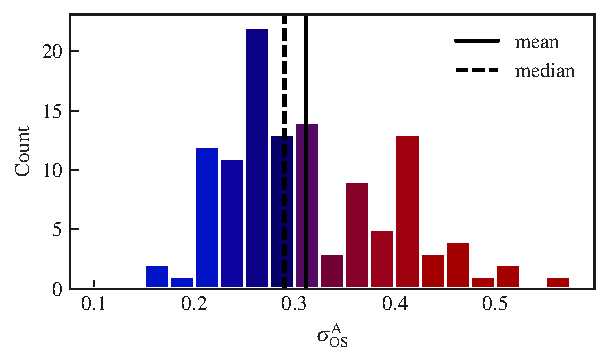
\includegraphics[width=4.1in]{./data/plots/dataset/histogram.pdf}
	\caption{
		Histogram of $\sigmaAOS$ values samples for the 118 chosen materials
	}
	\label{fig:anh.histogram}
\end{figure}
All values are given with respect to room temperature, as this is the regime where the most experimental reference is available to benchmark the aiGK method and to showcase the approach. In total, there are experimental reference values for 45 materials available, were we have discarded sources of questionable quality.

The materials come from these sources:
From Ramprasad: 41
From Toberer: 3
From Springer: 4
From Roekeghem: 9
From ICSD: 55
From Seko: 2
From AAPL: 4
